%%% EPS notes.

\documentclass{momento}

\usepackage{danielphysics}
%\usepackage{wasysym}
\title{Exploring Planetary Systems}
\author{Daniel Williams}

% \usepackage{zref-xr}
% \externaldocument{/home/astronomy/grg/project}

\providecommand{\Lag}{\mathcal{L}} %The Lagrangian

\begin{document}
\maketitle

\tableofcontents

These notes are based on the \textit{Exploring Planetary Systems}
course taught at the Unviersity of Glasgow during the 2014--2015
session.

\part{Spaceflight}
\label{part:spaceflight}

\chapter{The Rocket Equation}
\label{cha:rocket-equation}

\section{Derivation of the rocket equation}
\label{sec:deriv-rock-equat}

In order to change its momentum a rocket ejects mass; the Tsiolkovsky
rocket equation relates the complications of the changing mass and the
rocket's dynamics.  To analyse the motion of the rocket we start at
Newton's second law,
\begin{equation}
  \label{eq:10}
  \sum_i F_i = \dv{p(t)}{t}
\end{equation}
In the case of a rocket both the mass and the momentum have a time
dependence, and
\begin{equation}
  \label{eq:11}
  \dv{p}{t} = \lim_{\Delta t \to 0} \qty( \frac{p_2 - p_1}{\Delta t} )
\end{equation}
Consider $p_1 = (m + \Delta m) V$, and $p_2 = m(V + \Delta v) + \Delta
m V~e$, where $V~e$ is the velocity of the exhausted mass.

In the frame of an observer,
\[ V~e = V - v~e \]
thus 
\begin{align*}
  p_2 - p_1 &= m(V + \Delta v) + \Delta m (V-v~e) - (m+\Delta m) V \\
&= m \Delta v - \Delta m \ v~e
\end{align*}
let $\dd{m} = -\Delta m$, so
\begin{align*}
  \dv{p}{t} &= \frac{m \Delta v + v~e \dd{m}}{\Delta t} \\
&= m \dv{v}{t} + v~e \dv{m}{t} = m \dot{v} + v~e \dot{m}
\end{align*}
Since there are no external forces, and assuming that $v~e$ is
constant,
\begin{align*}
  F &= m \dot{v} + v~e \dot{m} = 0 \\
m \dot{v} &= - v~e \dot{m} \\
\Delta v &= \int v~e m \dd{m} 
\end{align*}
which gives
\begin{fequation}[Tsiolkovsky rocket equation]
  \label{eq:13}
\label{eq:rocket-equation}
  \Delta v= v~e \log( \frac{m_0}{m(t)} )
\end{fequation}
Now define the mass fraction as the proportion of the propellant which
has been expended,
\begin{definition}[Mass fraction]
  \label{def:mass-fraction}
  \[ M~f = 1 - \qty[ \frac{m(t)}{m_0}] \]
\end{definition}

\section{Thrust}
\label{sec:thrust}

If we make the assumption that $\dot{m}$ is constant, then
\[ m(t) = m_0 - \dot{m} t \]
and the total time for driven flight can then be found,
\begin{equation}
  \label{eq:14}
  t = \frac{m_0 - m(t)}{\dot{m}} = \frac{m_0}{\dot{m}} \qty( 1 - \frac{m}{m_0}) = \frac{m_0}{\dot{m}} M~f
\end{equation}
hence the range of the rocket is
\begin{align*}
  s(t) &= \int_0^t v(t') \dd{t'}\\ &= v~e \int_0^t \log( \frac{m_0}{m_0 - \dot{m} t'} ) \dd{t'} \\ &= v~e \frac{m_0}{\dot{m}}
\qty[\qty(1- \frac{\dot{m} t}{m_0}) \log( 1 - \frac{\dot{m} t}{m_0}) + \frac{\dot{m}}{m_0} t]\\
& \text{since } m(t) = m = m_0 - \dot{m} t, 1- \dot{m} t / m_0 = m(t)/m\\
&= v~e \frac{m_0}{\dot{m}} \qty[ \frac{m}{m_0} \log( \frac{m}{m_0}) +  1 - \frac{m}{m_0}] \\ 
&= v~e \frac{m_0}{\dot{m}} \qty[ 1 - \frac{m}{m_0} \qty( \log(\frac{m}{m_0}) + 1 )]
\end{align*}

\section{Equations of motion}
\label{sec:equations-motion}

We now have a set of equations to describe the rocket's motion,
\begin{align}
  \label{eq:15}
  v(t) &= v~e \log( \frac{m_0}{m} ) \\
  \label{eq:16}
  t &= \frac{m_0}{\dot{m}} M~f \\
  \label{eq:17}
  s(t) &= v~e \frac{m_0}{\dot{m}} \qty[1 - \frac{m}{m_0} \qty(\log( \frac{m}{m_0} )+1)] + v_i \frac{m_0}{\dot{m}} M~f
\end{align}

It is useful to define a new quantity here also:
\begin{definition}[Specific Impulse]
\label{def:specific-impulse}
  \[ I~{sp} = \frac{v~e}{g} \]
\end{definition}
which is just the exhaust velocity normalised by the gravitational
acceleration.

\begin{example}[A simple rocket]
  Consider the third stage burn of a rocket, which has an initial
  velocity $v~i = 2 \e{3}\, \meter\, \second^{-1}$, and contains $4
  \e{3}\, \kilogram$ of fuel, and has an empty mass of $700\,
  \kilogram$. The vacuum exhaust speed is $v~e =
  2930\,\meter\,\second^{-1}$, with
  $\dot{m}=100\,\kilogram\,\second^{-1}$. \\ How far does the rocket
  travel during the burn?  The mass ratio is $\frac{4.7}{0.7} =
  6.71$, so \[ \Delta v = v~e \log(6.71) =
  55.79\,\meter\,\second^{-1} \] and the burn time is
\[ \Delta t = \frac{4.7}{0.1 (1 - \frac{0.7}{4.7} )} \approx 40\,\second \]
Thus \begin{align*} s &= 2930\,\meter\second^{-1} &&\times \frac{4700\,\kilogram}{100\,\kilogram\,\second^{-1}}\\ &&& \times \qty[1 - \frac{1}{6.71} \qty( \log(6.71) + 1 )] \\&= 158.51 \kilo\meter 
\end{align*}
\end{example}

\section{Multistaging}
\label{sec:multistaging}

The structural mass of the rocket is a major source of inefficiency
during the burn, and one way to reduce its impact is to jettison
stages of the rocket as the fuel they are carrying is expended. This
allows a greater speed to be achieved with the same quantity of
fuel. Modern rockets seldom use more than three stages due to the
engineering compexity, however.

From the rocket equation (\ref{eq:rocket-equation}), we have
\[ v(t) = v~E \log( \frac{M_0}{M} ) + v~i \] for $M_0$ the initial
mass of the rocket, and $M$ its final mass, while $v~i$ is its
velocity at the start of the burn. For a single stage rocket the
velocity boost will be
\[ v(t) = v~E \log(R_0) \]
where 
\[ R_0 = \frac{M~S + M~f + M~p}{M~s + M~p} \] for $M~S$, $M~f$, and
$M~p$ respectively the masses of the structure, fuel, and payload.

If the rocket is composed of two stages with equal mass,
\[ v(t) = v~E \log(R_1) + v~E \log(R_2) \] which is larger than the
total speed achievable using a single-stage rocket.

%%% Local Variables: 
%%% mode: latex
%%% TeX-master: "../project"
%%% End: 


\chapter{Rocket Launches}
\label{cha:rocket-launches}

\section{Vertical motion against gravity}
\label{sec:vert-moti-against}

Consider a rocket with thrust velocity perpendicular to the
gravitational field. The force equation  is
\begin{equation}
  \label{eq:1}
  \dv{v}{t}= \frac{F-Mg}{M}
\end{equation}
For $Mg$ the instantaneous weight of the rocket. Hence
\begin{equation*}
  \label{eq:2}
  \dv{v}{t} = -v~E \frac{\dot{M}}{M}-g
\end{equation*}
then
\begin{equation*}
  \dd{v} = - v~E \frac{\dd{M}}{M} - g \dd{t}
\end{equation*}
and integrating both parts from $t=0$ to $t$,
\begin{equation*}
  v(t) = - v~E \int_{M_0}^M \frac{\dd{M'}}{M'} - \int_0^t g \dd{t'}
\end{equation*}
Assuming that $g$ is constant over the flight,
\begin{align*}
  v(t) &= v~E \log( \frac{M_0}{M(t)} )-gt \\
&= v~E \log(\frac{M_0}{M(t)}) - g \frac{M_0}{\dot{M}} \qty( 1 - \frac{M}{M_0})
\end{align*}
with the second part of the equation the gravity loss term.

\section{Thrust-to-weight ratio}
\label{sec:ttw-ratio}

In order to optimise the amount of energy lost due to gravity we can
consider the \emph{thrust-to-weight ratio}, 
\begin{equation}
  \label{eq:3}
  \psi = \frac{F}{g M_0} = \frac{v~E \dot{M}}{g M_0}
\end{equation}
which allows us to write
\begin{equation}
  \label{eq:4}
  \frac{v(t)}{v~E} = \log( \frac{M_0}{M(t)} ) - \frac{1}{\psi} \qty( 1 - \frac{M}{M_0} )
\end{equation}

\section{Vertical range}
\label{sec:vertical-range}

To calculate the vertical range of a rocket we proceed as before by
integrating the velocity over $t$
\begin{align*} 
s &= \int v(t) \dd{t} = v~E \int_0^t \log( \frac{M_0}{M(t)} ) \dd{t} - \int_0^t g t \dd{t'} \\
&=v~E \frac{M_0}{\dot{M}} \qty[ 1 - \frac{M}{M_0} \qty( \log( \frac{M_0}{M(t)}) + 1 ) ] - \half g t^2 \\
&=v~E \frac{M_0}{\dot{M}} \qty[ 1 - \frac{M}{M_0} \qty( \log( \frac{M_0}{M(t)}) + 1 ) ] \\ & \quad- \frac{g}{2} \frac{M_0^2}{\dot{M}^2} \qty( 1 - \frac{M}{M_0})^2
\end{align*} assuming $g$ is constant.

\section{Launch aspects}
\label{sec:launch-aspects}

Consider the kinetic energy of the payload,
\begin{align*}
  \half M \Delta v^2 &= \half M v~E^2 \log^2\qty(\frac{M_0}{M}) \\ &= \half M v~E^2 \log^2\qty(R)
\end{align*}
For $R$ the rocket parameter. Normalising this by the rest-frame
energy of the propellant in the rocket,
\[ \half (M_0-M) v~E^2 \]
we find the ratio
\begin{equation}
\label{eq:5} \phi(R) = \frac{M}{M_0-M} \log^2(R) = \frac{\log^2(R)}{R-1} 
\end{equation}

\begin{figure}[b]
  \centering
  \begin{tikzpicture}
    \begin{axis}[xmin=0, ymin=0, height = 5cm, width=\columnwidth, xlabel=$R$, ylabel=$\phi(R)$]
      \addplot[mark=none, draw=muted-green, ultra thick, domain=1:10] {(ln(x)*ln(x))/(x-1)};
    \end{axis}
  \end{tikzpicture}
  \caption{$\phi(R)$ as a function of the rocket parameter, $R$.}
  \label{fig:rocket-ratio}
\end{figure}

By differentiating we find the optimal $R$ to be
\begin{equation}
  \label{eq:6}
  \dv{\phi}{R} = 0 = - \frac{\log^2(R)}{(R-1)^2} + \frac{2 \log(R)}{R(R-1)}
\end{equation}
So the optimal $R = R~C$ satisfies
\begin{equation}
  \label{eq:7}
  \log{R~C} = 2 - \frac{2}{R~C}
\end{equation}
so $R~C \approx 4.9$.

%%% Local Variables: 
%%% mode: latex
%%% TeX-master: "../project"
%%% End: 


\chapter{Orbits \& Manoeuvres }
\label{cha:orbits}

\chapter{Rocket Engines}
\label{cha:rocket-engines}

\chapter{New Propulsion Methods}
\label{cha:new-prop-meth}



\part{Space Exploration}
\label{part:space-exploration}

\chapter{Detecting Exoplanets}
\label{cha:detecting-exoplanets}

A planet is an object which orbits a star or a stellar remnant,
defined in 2006 by the IAU as celestial body which
\begin{itemize}
\item is in orbit around the Sun,
\item has sufficient mass for its self-gravity to overcome rigid body
  forces so that it assumes a hydrostatic equilibrium (nearly round)
  shape, and
\item has cleared the neighbourhood around its orbit.
\end{itemize}
an exoplanet is a planet in orbit about a star other than our own.

The earliest attempts to detect exoplanets came from Huygens in 1698,
while the first successful detection was made in 1992, with the
discovery of a planet orbiting a pulsar. The first main sequence star
found to have planets was 50 Persei in 1995.

There are a number of methods used to detect exoplanets:

\begin{description}
\item[Direct observation] Planets are identified by the reflected
  radiation, either through optical, infra-red, or radio emission, and
  its polarisation.
\item[Doppler Method] Radial velocity changes of the star with respect
  to the Earth can be deduced from the star's spectral lines.
\item[Astrometry] By measuring the position of a star in the sky the
  'wobble' in the star's relative motion caused by the planet can
  reveal the presence of planets.
\item[Transit Method] The effect of the planet on the observed
  luminosity of a star as it passes in front of the disk can be
  measured.
\item[Gravitational Microlensing] The gravitational field of a star
  acts like a lens, brightening the background stars.
\item[Pulsar Timing] The presence of a planet introduces a delay in
  the arrival of pulses.
\end{description}

\section{Direct Observation}
\label{sec:direct-observation}

\subsection{Albedo}
\label{sec:albedo}

The albedo is the ability of an object to reflect light. \\
Let the radiation flux density on the surface of the Sun be $F~\sun$,
and so the flux density, $F~p(r)$ at a distance $r$ from the star is
\begin{equation}
  \label{eq:1}
  F~p(r) = F~\sun \frac{R^2_{\sun}}{r^2}
\end{equation}
with $R_{\sun} /\ r$ being the angular diameter of the Sun at a
distance $r$. Then the total flux on the surface of the planet then becomes 
\[ L = \pi R^2~p F~p = \pi R^2~p F_{\sun} \frac{R^2_{\sun}}{r^2} \]

\subsection{Bond Albedo}
\label{sec:bond-albedo}

The Bond Albedo, $A$, is defined as the ratio of the emergent flux to
the incident flux. The flux reflected by the planet is

\begin{equation}
  \label{eq:2}
  L = L^{\prime} \cdot A =  \pi R^2~p A F_{\sun} \frac{R^2_{\sun}}{r^2}
\end{equation}

If a planet is a distance $\Delta$ from the observer its observed
flux, $F$, will be
\begin{equation}
  \label{eq:3}
  F = \frac{L^{\prime}}{4 \pi \Delta^2}
\end{equation}

However, reflection is anisotropic, so the flux must be corrected by a
factor $C \Phi(\alpha)$ which depends on the phase angle of the
planet. The function $\Phi$ is the phase function, and is normalised
such that $\Phi(\alpha = 0) = 1$. We also require the normalising
constant $C$ such that
\begin{equation}
  \label{eq:4}
  \frac{ C \int_S \Phi(\alpha) \dd{S}}{4 \pi \Delta^2} = 1
\end{equation}

With this, the true observed flux at a distance $\Delta$ will be
\begin{equation}
  \label{eq:5}
  F = \frac{C \Phi(\alpha) L^{\prime}}{4 \pi \Delta^2} 
    = \frac{C \Phi(\alpha)}{4 \pi \Delta^2} A \pi R^2~p F_{\sun} \frac{R_{\sun}^2}{r^2}
\end{equation}

Now, since
\begin{align*}
  \int_S \Phi(\alpha) \dd{S} & = \Delta^2 \int_{\alpha=0}^{\pi} \int_{\phi=0}^{2\pi} \Phi(\alpha) \sin(\alpha) \dd{\alpha} \dd{\phi} \\
                             & = 2 \Delta^2 \pi \int_0^{\pi} \Phi(\alpha) \sin(\alpha) \dd{\alpha}                                   \\
  \therefore C               & = \frac{2}{\int_0^{\pi} \Phi(\alpha) \sin(\alpha) \dd{\alpha}}
\end{align*}

Let $q = \frac{CA}{4}$. The Bond Albedo, $A$, can be expressed
\begin{equation}
  \label{eq:6}
  A = 2 p \int_{\alpha=0}^{\pi} \Phi(\alpha) \sin(\alpha) \dd{\alpha}
\end{equation}
with $p$ the geometric albedo, and $q$ is the phase integral:
\begin{equation}
  \label{eq:7}
  q = 2 \int_{\alpha=0}^{\pi} \Phi(\alpha) \sin(\alpha) \dd{\alpha}
\end{equation}

\subsection{Geometric Albedo}
\label{sec:geometric-albedo-1}

A Lambertian surface is a perfectly white diffuse surface which
reflects all incident radiation, with a phase function $\Phi(\alpha) =
\cos(\alpha)$. Thus
\begin{equation}
  \label{eq:8}
  C = \frac{2}{\int_0^{\pi} \Phi(\alpha) \sin(\alpha) \dd{\alpha}} 
    = \frac{2}{\int_0^{\pi/2} \cos(\alpha) \sin(\alpha)  \dd{\alpha} } = 4
\end{equation}
which implies that $A = p = 1$ for a Lambertian surface.

We can then use a Lambertian surface to measure the amount of light
reflected from another surface.  Take the observed flux density,
equation (\ref{eq:5}), and let $\alpha=0$. Now take the flux density
of the Lambertian surface,
\begin{equation}
  \label{eq:9}
  F~L(\alpha=0) = \frac{4}{4 \pi \Delta^2} \pi R~p^2 F_{\sun} \frac{R_{\sun}^2}{r^2} 
\end{equation}
since $A=1$. The ratio of these two gives $\frac{F}{F~L} = p$.

\section{Astrometric detection}
\label{sec:astr-detect}

As a planet orbits a star the mutual gravitational force causes the
two to orbit a mutual barycentre, and as such, the star appears to
wobble from side to side. The motion of a single planet about a star
causes the star to undergo a reflex circular orbit about the
barycentre with a radius
\[ a~s = a \frac{M~p}{M~s} \] This results in periodic perturbation of
the radial velocity, astrometric position, and time of arrival of
periodic signals.

The Keck telescopes are capable of detecting the position of a star to
within $20\,\micro\text{as}$, which allows the barycentric motion to
be detected. The radius of the orbit about the barycentre for the star is
\begin{equation}
  \label{eq:26}
  r~s = r \qty( \frac{m~p}{m~s + m~p} ) \approx r \qty( \frac{m~p}{m~s})
\end{equation}
Thus, at a distance $d$ this will produce an angular movement of 
\begin{equation}
  \label{eq:27}
  \Delta \theta = \frac{r~s}{d} = \frac{r}{d} \frac{m~p}{m~s}
\end{equation}
Defining the mass ratio, $q = m~p/m~s$, then
\begin{equation}
  \label{eq:28}
  \Delta \theta = 0.5 \qty( \frac{q}{10^{-3}}) \qty( \frac{r}{5\,\text{AU}} ) \qty( \frac{d}{10\,\text{pc}})^{-1} \,\milli\text{as}
\end{equation}
This method has the advantage of being able to estimate the mass of a
planet, and is complementary to the spectroscopic method, as it works
best for face-on systems. It is also ideal for detecting planets with
long orbital periods. On the other hand, achieving the required
precision is difficult, and the method is highly sensitive to the
distance to the parent star. There are also periodic shifts in a
star's apparent centroid position due to dark regions on its surface,
so long observation times are needed to confirm a detection.

\section{Radial velocity}
\label{sec:radial-velocity}

In a system where the planet and star are, respectively at a distance
$r~p$ and $r~s$ from the barycentre the period will be
\[ P = \frac{2 \pi r~p}{v~p} = \frac{2 \pi r~s}{v~s} \] where $v~p$
and $v~s$ are the respective velocities. From conservation of momentum 
\[ M~p v~p = M~s v~s \] and so
\[ v~s = \frac{M~p}{M~s} \frac{2 \pi r~p}{P} \]
and since the line of sight may be inclined,
\[ v~r = v~s \sin(i) = \frac{M~p}{M~s} \frac{2 \pi r~p}{P} \sin(i) \]
is the radial velocity.

Recalling Kepler's third law,
\[ P^2 = \frac{4 \pi^2}{G(M~p + M~s)} r~p^3 \]
and so long as $M~p \ll M~s$,
\[ r~p \approx \qty( \frac{G M~s}{4 \pi^2} P^2 )^{\frac{1}{3}} \]
and therefore
\begin{equation}
  \label{eq:12}
  v~r = \qty( \frac{2 \pi G}{P})^{\frac{1}{3}} \frac{M~p}{M~s^{\frac{2}{3}}} \sin(i)
\end{equation}

The radial velocity can be measured from the Doppler shift of the
radiation from the star, and it is then possible to measure the
quantity $M~p \sin(i)$ for $i$ the inclination of the planet's
orbit. In the most general case the velocity amplitude, $K$, is
\begin{equation}
  \label{eq:18}
  K = \qty( \frac{2 \pi G}{P})^{\frac{1}{3}} \frac{M~p \sin(i)}{(M~p + M~s)^{\frac{2}{3}}} \frac{1}{(1-e^2)^{\half}}
\end{equation}
The star's mass can be estimated from the mass-luminosity
relationship, and once the distance to the star has been determined
(by parallax) the luminosity can be determined.

In absence of other constraints on the orbital inclination, radial
velocity searches can provide lower limits on the planetary masses of
a system. The magnitude of the radial velocity of the sun due to
Jupiter is around $12.5\,\meter/\second$, but due to the Earth is
$0.1\,\meter/\second$. The limit measurable by current instrumentation
is around $1\,\meter/\second$.

This method has the advantages of being independent of the distance to
the star, and the mass, period, and orbital elements of the planet can
be determined. It has the disadvantage of the inability to measure
$\sin(i)$ causing only the lower mass limit to be observable, thanks
to the SNR considerations around bright stars. Elliptical orbits
complicate the mathematics, as do multiple planet systems, and stellar
pulsations.

\section{Planetary transits}
\label{sec:planetary-transits}

A growing number of extra-solar planets are detected by the transit
method, whereby the photometric effect of the planet passing over the
star's disk is recorded. The dip in intensity is related to the area
of the two disks,
\begin{equation}
  \label{eq:19}
  \Delta I \propto \qty( \frac{R~p}{R~s} )^2
\end{equation}
for $R~p$ the radius of the planet and $R~s$ the radius of the star,
so a planet the size of Jupiter is likely to cause a 1\% drop in
intensity, whereas the Earth would only produce a 0.01\% drop.

The reduction in brightness can be found as the ratio of the
brightness during the transit to that outside the transit.
\begin{equation}
  \label{eq:20}
  \frac{B~s \pi (R~s^2 - R~p^2)}{B~s \pi R~s^2} = 1 - \qty( \frac{R~p}{R~s} )^2
\end{equation}
for $B~s$ the brightness of the star, and the fractional change,
$\Delta$ is then
\begin{equation}
  \label{eq:21}
  \Delta = \qty( \frac{R~p}{R~s} )^2
\end{equation}

The first transit observed was of a planet around HD\,209458, which
had a 2.5\,hour transit time. This method allows the radius of the
planet to be measured easily, and allows a simultaneous scan of a
large fraction of the sky, and allows the atmospheres of planets, and
satellites, to be studied. It does however, require a good alignment
between the planets' orbital plane and the observer, and produces a
high rate of false detections.

In order to determine the orbital period we can turn to Kepler's third
law. The radius of the star can be estimated from the star's spectral
classification, allowing the planet's radius to be estimated. Along
with the mass of the star and the period it is possible to find the
planet's orbital radius.

\begin{figure}[b]
  \centering
  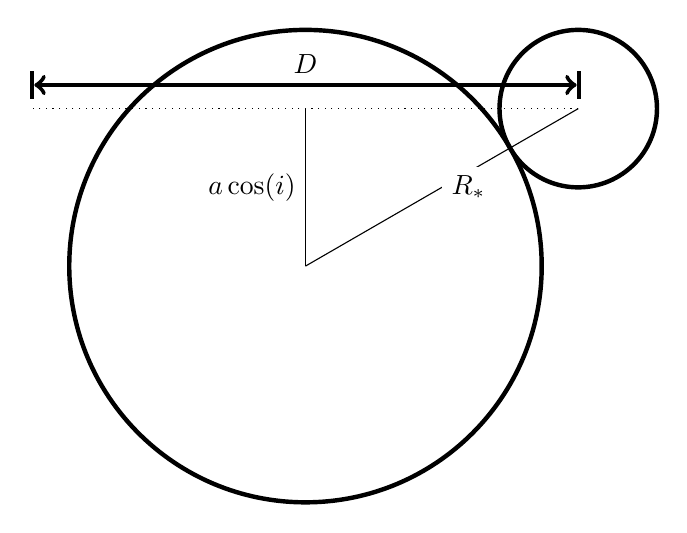
\begin{tikzpicture}[]
	\draw [ultra thick] ( 0,0) circle (3);
	\draw [ultra thick] (30:4) circle (1);
	\draw [dotted]   (30:4) -- (150:4);
	\draw [|<->|, ultra thick]     (-3.5, 2.3) -- (3.5,2.3) node [midway, above] {$D$};
	\draw (0, 0) -- (0,2) node [midway, left] {$a \cos(i)$};
	\draw (0,0) -- (30:4) node [midway, right, fill=white] {$R_*$};
\end{tikzpicture}
  \caption{The geometrical configuration of the transit.}
  \label{fig:transit-geometry}
\end{figure}

A transit will begin when the projected radius of the planet touches
the edge of the parent star, and lasts for a duration $\tau$ which is
a fraction of the total orbital period, and so the distance is a chord
of length
\begin{equation}
  \label{eq:22}
  D = 2 a \sin( \half \frac{2 \pi}{P} \tau) = 2 \sqrt{( R_{*} + R~p)^2 - a^2 \cos[2](i)}
\end{equation}
and so
\begin{equation}
  \label{eq:23}
  \tau = \frac{P}{\pi} \asin( \frac{\sqrt{(R_{*}+R~p)^2 - a^2 \cos[2](i)}}{a} )
\end{equation}
\begin{figure}[b]
  \centering
  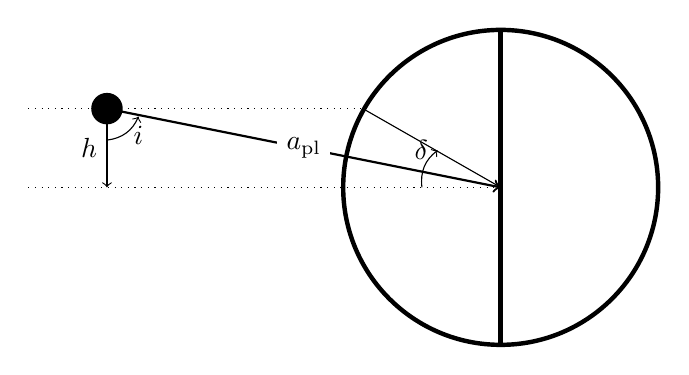
\begin{tikzpicture}[]
	\draw [ultra thick] (6,0) circle (2);
	\draw [ultra thick] (6,2) -- (6,-2);
	\draw [dotted]   (0,1) -- (4.25,1);
	\draw [dotted]   (0,0) -- (6,0);
	\draw [<->]      (1,0) -- (1,1) node [midway, left] {$h$};
	\fill (1,1) circle (0.2);
	\draw [thick, <->] (1,1) -- (6,0) node [midway,fill=white] {$a_{\rm pl}$};
	\draw [->] (1,0.6) to [bend right] (1.4,0.9) node [below] {$i$};
\draw (6,0) -- (4.25,1);
\draw [->] (5, 0) to [bend left] (5.2, 0.47) node [left] {$\delta$};
\end{tikzpicture}
  \caption{The transit geometry, side-on.}
  \label{fig:transit-geometry-2}
\end{figure}
This can also be described, using the geometry of figure
\ref{fig:transit-geometry-2} as
\begin{align*}
  \label{eq:24}
  \tau &= \frac{P}{\pi} \qty( \frac{R_{*} \cos(\delta) + R~p}{a} ) \\ &\approx 13 \qty( \frac{M_{*}}{M_{\odot}})^{-\half} \qty( \frac{1}{1\,\text{AU}} )^{\half} \qty( \frac{R_{*}}{R_{\odot}} )
\end{align*}
We find that the appropriate transit period is around 13 hours and 25
hours for Jupiter.

In order to view a transit the inclination of the system must
satisfy \[ \cos(i) \le \frac{(R~p + R~s)}{a} \] and the probability of
viewing a transit for the system is
\begin{equation}
  \label{eq:25}
  P(\text{transit}) = \frac{\int_0^{(R~p+R~s)/a} \dd{\cos(i)}}{\int_0^1 \dd{\cos(i)}} = \frac{R~p + R~s}{a} \approx \frac{R~s}{a}
\end{equation}

\section{Gravitational microlensing}
\label{sec:grav-micr}

If a planet aligns precisely with the line-of-sight then the image of
the star will be deformed into a circle with a radius
\begin{equation}
  \label{eq:30}
  \theta~E = \sqrt{ \frac{4 G M~L}{c^2 D~L} \frac{(D~S - D~L}{D~S}} }
\end{equation}
This comes from the angle of deviation caused by the lens,
\begin{equation}
  \label{eq:29}
  \alpha = \frac{4 G M~L}{c^2 r} = \frac{2 R~s}{r}
\end{equation}
for $R~s$ the Shcwarzschild radius, and $r$ the distance of closest
approach, and $M~L$ is the mass of the lens. For a full derivation see
notes on \textsc{General Relativity} for more information.

The total magnification, $A$, which is produced is
\begin{equation}
  \label{eq:31}
  A = \frac{u^2 + 2}{u \sqrt{u^2 + 4}}
\end{equation}
where $u = \theta~s / \theta~E$ is a dimensionless unit representing
the source-lens separation in units of the Einstein radius. The
characteristic time of a lensing event is
\begin{equation}
  \label{eq:32}
  t~E = 69.9 \qty( \frac{M~L}{M_{\odot}} )^{\half} \qty( \frac{D~S}{8\,\kilo\text{pc}})^{\half} \qty[ (1-d)d]^{\half} v^{-1}_{200}\,\text{days}
\end{equation}

\textbf{A better description is contained in Dominik and Sahu, worth
  writing up from there.}

This method has the advantage of allowing the detection of Earth-like
planets, and allows a distribution of planetary systems to be
measured. Unfortunately lensing is a one-off process, and planets are
distant, so follow-up observations are implausible.

\section{Pulsar timing}
\label{sec:pulsar-timing}



%%% Local Variables: 
%%% mode: latex
%%% TeX-master: "../project"
%%% End: 


\onecolumn
\chapter{Distribution of Exoplanets}
\label{cha:distr-exopl}
\section{Mass distribution}
\label{sec:mass-distribution}
\includegraphics{figures/masshist.pdf}
\includegraphics{figures/massyear.pdf}
\includegraphics{figures/eccmass.pdf}
\includegraphics{figures/semimass.pdf}

\section{Semi-major axes}
\label{sec:semi-major-axes}

\includegraphics{figures/axishist.pdf}
\includegraphics{figures/eccsemi.pdf}

% \section{Atmospheres}
% \label{sec:atmospheres}

% HD\,209458\,b was the first planet to have a spectroscopic signature
% of sodium discovered in its atmosphere, but at an intensity lower than
% was expected, suggesting that high clouds obscure the lower layers of
% the atmosphere. The planet's spectrum is extracted by subtracting the
% stellar spectrum from the overall spectrum.

%%% Local Variables: 
%%% mode: latex
%%% TeX-master: "../project"
%%% End: 

\twocolumn

\chapter{Formation of Planetary Systems}
\label{cha:form-plan-syst}
In our Solar System all of the planets orbit anticlockwise, with the
sun rotating in the same direction, and all of the orbital planes are
close to coplanar (except Mercury). Their orbits are very close to
circular (except Mercury, with $e=0.2$), and with the exception of
Venus and Uranus, they all rotate anticlockwise. Each planet is
approximately twice the distance from the sun of the previous one, and
most satellites orbit anticlockwise.

\section{The nebular hypothesis}
\label{sec:nebular-hypothesis}

In the nebular hypothesis the sun and planets formed from a cloud of
interstellar material, with the sun forming at the centre of a
flattened high density region. The planets then form out of the
remainder of the cloud. There are a number of questions arising from
this idea though. How does a lat solar system form, and how do the
planets form?

The Jeans criterion states that compressive perturbations of a gas
with uniform density, $\rho$, and sound speed $c~s$ over distances
greater than the Jeans length, $\Lambda$,
\begin{equation}
  \label{eq:35}
  \Lambda = \qty( \frac{\pi c~s^2}{G \rho})^{\half}
\end{equation}
where $G$ is the gravitational constant. For a one solar mass cloud
core with a temperature of $10\,\kelvin$ and a radius of
$0.1\,\text{pc}$ this occurs over a timescale of around one million
years

Radio measurements of gas clouds show that they do possess angular
momentum, and have rotational periods of around 20 million years. The
centrifugal force per unit mass of the gas is then $j^2/r^3$, for $r$
the distance from the axis, and so the elements are balanced within a
disk.

\section{Evolution of  a stellar nebula}
\label{sec:evol-astell-nebula}

Consider the condition for centrifugal balance,
\begin{equation}
  \label{eq:36}
  \frac{j^2}{r^3} = \pdv{\Phi}{r}
\end{equation}
where the gravitational force is 
\[ - \pdv{\Phi}{r} \]
so the energy of an element of gas, per unit mass, is
\begin{equation}
  \label{eq:37}
  E = \frac{j^2}{2r^2} + \Phi
\end{equation}
Thus the change of total energy due to interaction between two gas
elements is
\begin{equation}
  \label{eq:38}
  \dd{E} = \frac{j_1 \dd{j_1}}{r^2} - \frac{j_1^2 \dd{r_1}}{r_1^3} + \dd{\Phi_1} + \frac{j_2 \dd{j_2}}{r^2} - \frac{j_2^2 \dd{r_2}}{r_2^3} + \dd{\Phi_2}
\end{equation}
Considering the conservation of momentum, and the balance of forces,
\begin{equation}
  \label{eq:39}
  \dd{E} = \qty( \frac{j_1}{r^2} - \frac{j_2}{r^2} )\dd{j_1} = \qty( \Omega_1 - \Omega_2 ) \dd{j_1}
\end{equation}
Planets form through a multi-step process, with solid grins condensing
out of the gas of the nebula, which accrete into larger bodies:
planetesimals, which then collide and coalesce to form protoplanets.

Dust particles then start to settle into the plane of the
protoplanetary disk, with the gravitational force in the $z$-direction
being
\begin{equation}
  \label{eq:40}
  \frac{GM m~g z}{R^3}
\end{equation}
where $R$ is the distance of the grain from the star, and $m~g$ is its
mass. The angular velocity will then be
\begin{equation}
  \label{eq:41}
  \Omega^2 = \frac{GM}{R^3}
\end{equation}
so the acceleration on each grain is
\begin{equation}
  \label{eq:42}
  g_z = \Omega^2 z
\end{equation}

As each dust particle falls towards the centre of the disk it
experiences drag from the gas it travels through. For a spherical
particle of radius $a$ travelling at a velocity $v$ through a gas of
density $\rho$ this drag is
\begin{equation}
  \label{eq:43}
  F~{drag} = \pi a^2 \rho c~s v
\end{equation}
for $c~s$ the sound speed of the gas. The equation of motion for the
grain is then
\begin{align}
  m~g \dv{v}{t} &= F~{drag} - m~g g_z \\
\frac{4 \pi a^3 \rho~g}{3} \dv{v}{t} &= \pi a^2 \rho c~s v - \frac{4 \pi a^3 \rho~g}{3} \Omega^2 z
\end{align}
for grains of density $\rho~g$.

At some point the grain will reach a terminal velocity, when its
acceleration reaches $0$, so
\begin{equation}
  \label{eq:44}
  v = \frac{4 a \rho~g \Omega^2 H}{3 \rho c~s} \sim \frac{4 a \rho~g \Omega}{3 \rho} \sim \frac{8 a \rho~g \Omega H}{3 \Sigma}
\end{equation}
for $z=H$, the scale height of the disk from its mid-point, an
isothermal sound speed, $c~s \approx H \Omega$, and $\Sigma$ the
surface density, $\Sigma = 2 H \rho$. The settling time is then
\begin{equation}
  \label{eq:45}
  \tau~s \sim \frac{H}{v} \sim \frac{3 \Sigma}{8 a \rho~g \Omega} \sim \frac{\Sigma}{16 a \rho~g}\,\text{orbits}
\end{equation}
For $\Sigma \sim 10^3\,\kilogram\,\meter^{-2}$, $\rho~g \sim
10^3\,\kilogram\,\meter^{-3}$, $a = 10^{-5}\,\meter$, we get $10^4$
orbits, or $10^5$ years at a distance $5\,\text{AU}$.

\section{The formation of planetessimals}
\label{sec:form-plan}

Dust particles collide and coalesce in the midplane of the disk, and
in the time scale of the settling time they grow into objects with a
radius of between $1$ and $1000\,\kilo\meter$, at which point the
gravitational effect of the objects becomes significant. Each
planetessimal will sweep up material about a radius $r$, and so
accrete matter at a rate
\begin{equation}
  \label{eq:46}
  \dv{m~c}{t} = v_0 n m \pi r^2
\end{equation}
for particles of initial velocity $v_0$, number density $n$, and mass
$m$. By conservation of energy,
\begin{align*}
  \half m v_0^2 &= \half mv^2 - \frac{Gm~c m}{R~c} \\ 
v^2 &= v_0^2 + \frac{2 G m~c}{R~c} \\
v &= \sqrt{v_0^2 + \frac{2G m~c}{R~c}} \\
\dv{m~c}{t} &= v_0 n m \pi R~c^2 \qty( 1 + \frac{2 G m~c}{R~c v_0^2} )
\end{align*}

The timescale for the planetesimal to double its mass is
\begin{equation}
  \label{eq:47}
  \tau~{double} = m~c \qty( \dv{m~c}{t})^{-1}
\end{equation}
From the previous expression we can see when $Gm~c / R \approx v_0^2$,
this is proportional to $m~c^{1/3}$, and so smaller planetesimals grow
faster than large ones, and we have orderly growth. However, when
$Gm~c / R~c \gg v_0^2$ the gravitational force domiantes and $\tau~c
\propto m~c^{-1/3}$, and we have runaway growth.

\section{Isolation mass}
\label{sec:isolation-mass}

The next consideration is how large a planetary embryo can grow by
accreting other planetesimals. To find this, define an annulus of
half-width
\[ \Delta a~{max} = C R~{Hill} \] for $R~{Hill}$ the radius of the
Hill sphere where the embryo's gravitational influence dominates its
parent star, with
\begin{equation}
  \label{eq:48}
  R~{Hill} = a \qty( \frac{m~c}{3 M_{*}} )^{\frac{1}{3}}
\end{equation}
The isolation mass, where accretion stops, with $\Sigma~s$ the surface density of planetesimals, and $a$ the semimajor axis of the orbit, is
\begin{equation}
  \label{eq:49}
  m~{iso} = 2 \pi a \Sigma~s \Delta a~{max}
\end{equation}
Substituting in the half-width
\begin{align*}
  m~{iso} &= 2 \pi a \Sigma~s \Delta a~{max} \\
&= 2 \pi a \Sigma~s C a \qty( \frac{m~{iso}}{3 M_{*}} )^{1/3} \\
&= \sqrt{8 \pi^3} a^3 \Simga~s^{\frac{3}{2}} C^{\frac{3}{2}} \qty( 3 M_{*})^{- \frac{1}{2}}
\end{align*}
Them, taking $C=2 \sqrt{3}$, $\Sigma~s = 100\,\kilo\gram\,\meter^{-2}$
at $a = 1\,\text{AU}$, $m~{iso} = 0.07 M~E$. Thus terrestrial planets
did not form simply by embryos accreting matter, but this model is in
line with the estimated core masses of Saturn, Neptune, and
Uranus. For terrestrial planets the perturbations of the outer planets
are likely to have been significant.

\section{Formation of gas giants}
\label{sec:formation-gas-giants}

The core accretion model for gas giant formation is favoured, but a
second, gravitational instability model also exists.

\subsection{Core accretion}
\label{sec:core-accretion}

In the core accretion model a gas giant starts as the rock and ice
planetary embryo considered in the previous model, but this core
becomes so large that it is capable of supporting a gas envelope,
which remains at hydrostatic equilibrium until it reaches a critical
mass (around $15\,M~E$), after which it contracts on the
Kelvin-Helmholtz timescale (around $10^6$ years). After this a phase
of rapid gas accretion occurs until the planet is sufficiently massive
to open a gap in the protoplanetary disk. Radial planetary migration
can change the timescale of this process however.

The critical mass can be found from the relation
\begin{equation}
  \label{eq:50}
  \frac{M~{crit}}{M~E} \approx 12 \qty( \frac{\dot{M}~{core}}{10^{-6}\,M~e/\text{year}} )^{\frac{1}{4}} \qty( \frac{\kappa~R}{1\,\centi\meter\,\gram^{-1}} )^{\frac{1}{4}}
\end{equation}
for $\kappa~R$ the Rosseland mean opacity across all frequencies,
weighted by a Planckian distribution.

\subsection{Gravitational instability model}
\label{sec:grav-inst-model}

In this model the self-gravity of the gas in the protoplanetary disk
is sufficient to cause the disk to fragment and form clusters which
can then form gas giants. For this to work a high surface density is
required, which is most likely to occur early in the evolution of the
disk, and there are doubts as to whether there is sufficient time for
gas giants to form in this period. This model also favours the
formation of the planets at large radii (50 to 100\,AU).

For a rotating disk the Toomre $Q$-parameter quantifies the stability
of a system; for gravitational instability 
\[ Q \equiv \frac{c~s \Omega}{\pi G \Sigma} \lesssim 1 \] Taking the
speed of sound to be $c~s \simeq 0.5\,\kilo\meter/\second$ we would
require $\Sigma \approx 1.4\e{3}\,\gram\,\centi\meter^{-2}$. Assuming
a characteristic wavelength for a gravitational instability to be
\[ \lambda~{crit} = \frac{2 c~s^2}{G \Sigma} \]
then the mass of objects formed through disk fragmentation would be 
\[ M~p \sim \pi \Sigma \lambda~{crit}^2 \sim \frac{4 c~s^4}{G^2
  \Sigma} \sim 3\,M~J \] Approaching the point of fragmentation the
disk is likely to start forming spiral arms due to differential
rotation, allowing heat to transfer through the gas faster, increasing
the sound speed, and transferring angular momentum, leading to a lower
surface density. This the cooling time is an important
consideration. For the annulus of the disk the Kelvin-Helmholtz time
scale is
\[ t~{cool} = \frac{U}{2 \sigma T~{disk}^4} \] for $U$ the thermal
energy per unit surface area of the disk. If the cooling time is less
than the rotation period the heat can be radiated away and the disk is
likely to collapse.

\section{Planetary migration}
\label{sec:planetary-migration}

Planets will not necessarily remain in the orbits they formed in, and
orbits can change due to perturbations from larger planets,
interactions with planetesimals, and mutual interactions between
planets within the system.

As the newly formed planet interacts with the gas disk the gas can
develop vorticity, producing waves of higher gas density. These can
impart angular momentum on a planet if the have the same frequency as
the planet's gravitational potential, setting up a resonance. Density
waves from behind will exert a torque on the planet greater than the
torque from waves within the planet's orbit, forcing it into a lower
orbit. This is type I gas disk migration.

Type II gas disk migration occurs when high-mass planets interact
tidally with the gas disk as they accrete material. This tidal force
strongly perturbs the disk, and the exchange of angular momentum
between the planet and disk repels gas from the orbit, sweeping out an
annular gap in the gas disk. The planet will now move radially inward
as it accretes matter, and stops when it reaches the inner edge of the
gap. When a planet is large enough to open a gap orbital evolution
will occur; the radial velocity of the gas disk is
\[ v~r = -\frac{\dot{M}}{2 \pi r \Sigma} \] If there i a tidal barrier
on the outer edge of the gap the evolution of the disk will cause the
orbit to shrink provided that the local disk mass exceeds the planet's
mass. The rate of orbital shrinkage is equal to the radial velocity,
so the timescale is
\begin{equation}
  \label{eq:51}
  \tau_0 = \frac{2}{3 \alpha} \qty( \frac{h}{r} )^{-2} \Omega^{-1}
\end{equation}


%%% Local Variables: 
%%% mode: latex
%%% TeX-master: "../project"
%%% End: 


\chapter{Astrobiology}
\label{cha:astrobiology}
In order to determine which planets, and what conditions, are likely
to support life we need a firm concept of the concept of life.

\section{Life}
\label{sec:life}

Terrestrial life is based on a number of organic molecules, composed
primarily from hydrogen, carbon, oxygen, and nitrogen. These include
fatty acids, carbohydrates, and amino acids. These elements are fairly
abundant in the universe: hydrogen exists as a result of the big bang,
oxygen is synthesised in core-collapse supernovae, and carbon and
nitrogen (and oxygen) are synthesised in the CNO process. As we know
it, life also requires a terrestrial planet with liquid water. This
requires a temperature in the range $270$ to $370\,\kelvin$, and a
sufficiently high atmospheric pressure to support it.

\section{Equilibrium temperature}
\label{sec:equil-temp}

The emission of stars and planets can be approximated as blackbody
radiation, so, the flux from a body at temperature $T$ is
\begin{equation}
  \label{eq:52}
  F = \sigma T^4
\end{equation}
for $\sigma$ the Stefan-Boltzmann constant, the total radiative power
is then
\begin{equation}
  \label{eq:53}
  P = 4 \pi R~p^2 \sigma T^4~p
\end{equation}
and a planet at a distance $r~p$ absorbs
\begin{equation}
  \label{eq:54}
  P = (1-A) \pi R~p^2 \qty( \frac{R_{\odot}}{r~p} )^2 \sigma T^4_{\odot}
\end{equation}
for an albedo, $A$, of the planet. Equating these,
\begin{equation}
  \label{eq:55}
  T~p = (1-A)^{\frac{1}{4}} \qty( \frac{R_{\odot}}{2 r~p} )^{\half} T_{\odot} \approx 279 (1-A)^{\frac{1}{4}} r~p^{-\half}
\end{equation}
So, for a general star of luminosity $L$,
\begin{equation}
  \label{eq:56}
  T~p = \qty( \frac{(1-A)L}{16 \pi \sigma r~p^2} )^{\frac{1}{4}}
\end{equation}

\section{The greenhouse effect}
\label{sec:greenhouse-effect}

The greenhouse effect can be incorporated by adding a term $\Delta T$
to equation (\ref{eq:56}). This is a result of the absorption of
infrared radiation which heats the atmosphere and in turn the surface
of the planet.

\section{Albedo}
\label{sec:albedo-1}

The terrain and atmosphere contribute strongly to the albedo of a
planet. For example for snow $A \approx 0.8$.

\section{Stability of the atmosphere}
\label{sec:stability-atmosphere}

A gas in thermodynamic equilibrium has a Maxwellian distribution of
velocities,
\[ F(v) \dd{v} \propto \exp( - \frac{m v^2}{2 kT} ) v^2 \dd{v} \]
and an average kinetic energy per particle
\[ \ev{T} = \frac{m}{2} \ev{v^2} = \frac{3 kT}{2} \]
so a root mean square velocity
\[ \ev{v^2}^{\half} = \qty(\frac{3kT}{m})^{\half} \] The escape
velocity of a planet is
\[ v~e = \sqrt{\frac{2GM}{R}} \]
so to retain an atmosphere in the long term 
\begin{equation}
  \label{eq:57}
  T \le \frac{GMm}{150 k R} 
\end{equation}
for a species of mass $m$, and assuming that the $v~e > 10 v~{rms}$.

%%% Local Variables: 
%%% mode: latex
%%% TeX-master: "../project"
%%% End: 



\appendices


\bibliographystyle{authordate1}
\bibliography{bibliography/planetary-systems}
\nocite{*}


\end{document}



%%% Local Variables: 
%%% mode: latex
%%% TeX-master: t
%%% End: 
